\chapter{Evaluación del descriptor HOG}
Para esta primera parte de la práctica se realizará un análisis de los resultados obtenidos con el descriptor HOG (Histogram of Gradients), para ello, se definirán diferentes funciones, tanto para entrenar el modelo y obtener resultados como para hacer validación cruzada. El contenido que se va a explicar a continuación se encuentra dentro de los archivos \textbf{Extracción de rasgos.py} y \textbf{pruebas\_hog.py}.

\section{Lectura de imágenes,creación del modelo y predicción con nuevas imágenes}
Lo primero que se debe hacer es leer los datos, para ello se ha creado la función \textit{loadTrainingData()}, esta función se encarga de abrir cada una de las imágenes contenidas en la carpeta de train que se proporciona con la práctica de ejemplo \textit{ECI.Practica}; por cada una de la imágenes se computa se descriptor HOG; para ello se hace uso de la función \textit{cv2.HOGDescriptor().compute()}. \\

Para esta práctica se está utilizando un descriptor HOG con parámetros por defecto; este descriptor por defecto utiliza un tamaño de ventana de 128x64, bloques de 16x16, desplazamientos de 8x8, ... Con estos parámetros obtenemos por cada ventana 3780 características. Las imágenes que se utilizan en esta práctica son de 128x64, por lo que al utilizar el descriptor sobre estas cada una producirá un vector con 3780 características. Además de computar el descriptor por cada una de las imágenes, se añaden también a un vector la clase a la que pertenece cada imagen; dicho vector contiene unos (imágenes con personas en las fotos) y ceros (imágenes con fondo, sin personas). Una vez se han generado todas las imágenes se devuelve una matriz que contiene todos los descriptores calculados y un vector con la clase de cada imagen. \\

Tras esto, se debe entrenar un modelo para después poder predecir clases de una imagen dada; para ello, se utilizará como clasificador un \textit{SVM} contenido en la librería de \textit{OpenCV}. Este clasificador permite utilizar diferentes tipos de ``kernels`` que se utilizan después para realizar transformaciones a los datos y conseguir una mejor separación de estos; por el momento se va a utilizar un kernel lineal, más tarde se realizarán pruebas con diferentes kernels y se analizarán los resultados obtenidos.\\

Para utilizar este clasificador es necesario utilizar la función \textit{cv.ml.SVM\_create()}, esta función nos genera un \textit{SVM} vacío al que le podemos aplicar los parámetros que queramos, por defecto se definirá el tipo de kernel (lineal) y el tipo de SVM (en este caso de clasificación); también se le pueden (o deben) añadir más parámetros dependiendo del tipo de kernel que se utilice. Una vez definidos dichos parámetros del \textit{SVM} se utiliza la función \textit{train()} a la que se le pasa la matriz de descriptores, el vector de clases de las imágenes y además se le añade un parámetro indicando si las filas son los ejemplos o son las columnas (en el caso de esta práctica son las filas las que contienen cada uno de los ejemplos). Todo esto está contenido dentro de la función \textit{train()}, definida dentro de la práctica, a la cual se le pasa la matriz de descriptores, el vector de clases, el tipo de kernel que utilizará el clasificador, y un parámetro llamado ``degree`` utilizado por algunos kernels. \\

Una vez se ha entrenado el modelo, podemos utilizarlo para predecir la clase de una imagen. Para ello se ha creado la función \textit{test()}, a la cual se le pasa una imagen y el clasificador que queremos utilizar. Para la imagen dada se computa su descriptor HOG; tras esto, se utiliza la función \textit{clasficador.predict()} para obtener la predicción; este método nos devuelve una tupla, de la cual nos interesa el segundo valor de esta, en la cual se encuentra un vector con la clase predicha para la imagen; si se utilizara la función \textit{clasificador.predict()} sobre varios descriptores, este vector contendría la clase predicha para cada uno de los descriptores. \\

El proceso de crear leer las imágenes, crear un modelo y realizar una prueba con una imagen esta contenido dentro de la función \textit{ejemploClasificadorImagenes()} dentro de este ejemplo se utiliza como test una imagen de una persona, por lo que el resultado de la predicción debe de ser uno. A continuación se mostrará la imagen utilizada y una foto con la salida de la función. \\

\newpage

\begin{figure}[H]
	\centering
	\subfigure{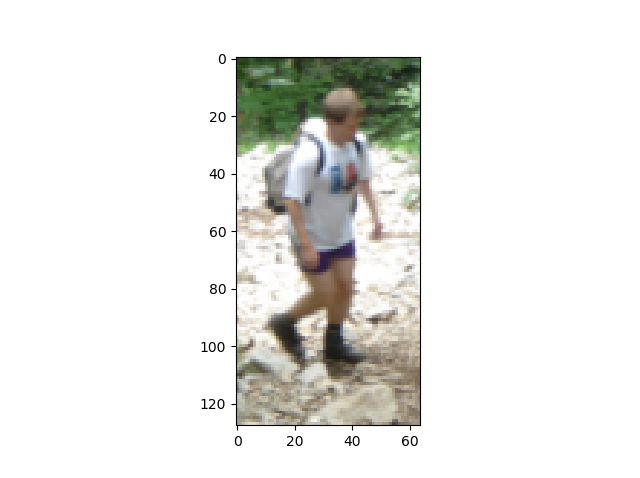
\includegraphics[width=80mm]{imagenes/prueba_img}}
	\subfigure{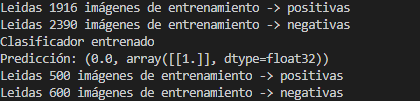
\includegraphics[width=80mm]{imagenes/resultado_ini}}
	\caption{Ejemplo clasificación con SVM lineal}
	\label{fig:salida_1}
\end{figure}

\section{Cálculo de medidas de interés para HOG}
En este apartado, se describirá el proceso realizado para obtener medidas de interés sobre el clasificador, para ello se cargará un conjunto de imágenes de test y se creará una función para calcular diferentes medidas de interés. \\

Para cargar el conjunto de imágenes de test se realiza el mismo proceso que en el apartado anterior, pero en vez de computar el descriptor para estas imágenes se guardan las imágenes; esto se realiza en la función \textit{loadTestData()}. Tras esto se utiliza la función \textit{test()} sobre cada una de las imágenes y se obtienen las predicciones del clasificador. Una vez se han obtenido las predicciones estás se guardan en un vector y se utiliza la función \textit{calculateMetrics()} para obtener las diferentes medidas. \\

La función \textit{calculateMetrics()} se encarga de obtener medidas de interés para los datos que se predicen, dichas medidas son \textit{F1-score}, \textit{Accuracy}, \textit{Precision}, \textit{True Negative Rate}, \textit{True Positive Rate}.A esta función se le debe pasar la predicción hecha por el clasificador y la clase real de los datos. Dichas medidas miden lo siguiente:
\begin{itemize}
	\item \textbf{Accuracy:} mide el porcentaje de predicciones correctas sobre el total de predicciones realizadas.
	\item \textbf{Precision:} mide el porcentaje de predicciones positivas reales sobre el total de predicciones positivas realizadas, es decir, el porcentaje de imágenes que se han clasificado como positivas que realmente son positivas.
	\item \textbf{True Positive Rate:} mide el porcentaje de predicciones positivas hechas sobre el total de datos positivos que hay, es decir, el porcentaje de imágenes positivas que se han clasificado como positivas.
	\item \textbf{True Negative Rate:} mide el porcentaje de predicciones negativas hechas sobre el total de datos negativos que hay, es decir, el porcentaje de imágenes negativas que se han clasificado como negativas.
	\item \textbf{F1-score:} está medida calcula una proporción entre \textit{Precision} y \textit{True Positive Rate}, indica la calidad de la predicción de la clase positiva, en nuestro caso sería detectar a una persona en la imagen. Esta medida decrece sin cualquiera de las dos medidas anteriores decrece.
\end{itemize}

Estas medidas nos serán útiles para conocer mejor como se está ajustando el clasificador entrenado con los datos. Los resultados obtenidos para nuestro conjunto de test son los siguientes.
\begin{figure}[H]
	\centering
	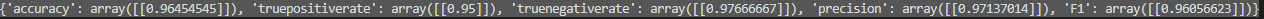
\includegraphics[width=140mm]{imagenes/resultados_test}
	\caption{Resultados de test para HOG}
	\label{fig:salida_2}
\end{figure}

Como se puede ver, los resultados son bastante buenos, obteniendo un 96\% aproximado de acierto, como se puede ver en el resto de medidas, el clasificador ha obtenido mejores resultados clasificando imágenes como fondo que como persona, aunque realmente no hay mucha diferencia.

\section{Pruebas con HOG}
En este apartado se compararán diferentes clasificadores a través de las medidas de interés descritas en el apartado anterior. Para este apartado se han utilizado todas las imágenes, en total 5406, y se ha utilizado validación cruzada para crear diferentes conjuntos de validación, de esta forma se pueden ver resultados más generales que no dependan solamente de los resultados de un único conjunto de validación y estar más seguros de la calidad del clasificador.\\

Para realizar validación cruzada se ha creado la función \textit{crossValidation()} esta función tiene como parámetros la matriz de datos con los descriptores, el vector de clases de dichos casos y el número de validaciones a realizar, por defecto este último parámetro es 5, el cual es el número de validaciones que se han utilizado para realizar el estudio de los diferentes clasificadores. También tiene parámetros adicionales para poder definir las características del clasificador. Dentro de esta función se realiza el siguiente proceso por cada validación.
\begin{enumerate}
	\item Se crea un conjunto de datos de validación. Para ello se utiliza la función de la librería \textit{sklearn.train\_test\_split()}; dicha función nos divide el conjunto de datos en un conjunto de datos de train y otro de test; para ello elige de forma aleatoria cada vez un conjunto de datos para test y forma el conjunto de train sin incluir dichos datos. Para el estudio se ha utilizado un tamaño de train del 80\% de los datos y un 20\% para test.
	\item Se crea un modelo y se entrena con el conjunto de datos de test.
	\item Se obtienen las predicciones de este modelo para los datos de test, se calculan la medidas anteriormente descritas y se guardan.
	\item Se actualiza el mejor modelo obtenido hasta el modelo, para ello se utiliza la medida \textit{Accuracy}; esto nos será útil para guardar el mejor modelo encontrado para la validación y utilizarlo más tarde si es necesario.
\end{enumerate}


Ahora, pasaremos a comentar los resultados obtenidos por el descriptor HOG con diferentes kernels de SVM y variando algunos parámetros. Los clasificadores que se han entrenado son los siguientes: SVM con kernel lineal, SVM con kernel radial (RBF), SVM con kernel polinómico con grados 2, 3, 4 y 5, SVM con kernel sigmoidal, SVM con kernel Chi Cuadrado y SVM con kernel Inter. Para cada uno de los modelo se han realizado 5 validaciones. Los parámetros a excepción de los diferentes clasificadores son los que hay por defecto; esto se ha hecho así para evitar ajustar los parámetros a un tipo de descriptor, ya que con otros descriptores; como los que se verán más adelante, los resultados pueden no ser justos por dichos parámetros .Los resultados son los siguientes:

\vspace{0.09in}

\begin{table}[H]
	\begin{tabular}{llllll}
		\textbf{Validation} & \textbf{F1} & \textbf{accuracy} & \textbf{precision} & \textbf{truenegativerate} & \textbf{truepositiverate} \\
		0                   & 0.955533    & 0.960259          & 0.966527           & 0.973019                  & 0.944785                  \\
		1                   & 0.960566    & 0.963956          & 0.979381           & 0.982699                  & 0.942460                  \\
		2                   & 0.959474    & 0.965804          & 0.962637           & 0.972756                  & 0.956332                  \\
		3                   & 0.953751    & 0.958410          & 0.960663           & 0.967905                  & 0.946939                  \\
		4                   & 0.970854    & 0.973198          & 0.979716           & 0.982759                  & 0.962151                 
	\end{tabular}
	\caption{Validación con SVM kernel lineal}
	\label{table_1}
\end{table}

\begin{table}[H]
	\begin{tabular}{llllll}
		\textbf{Validation} & \textbf{F1} & \textbf{accuracy} & \textbf{precision} & \textbf{truenegativerate} & \textbf{truepositiverate} \\
		0                   & 0.853179    & 0.882625          & 0.960938           & 0.975042                  & 0.767152                  \\
		1                   & 0.834146    & 0.874307          & 0.957983           & 0.975767                  & 0.738661                  \\
		2                   & 0.850123    & 0.887246          & 0.971910           & 0.983974                  & 0.755459                  \\
		3                   & 0.854237    & 0.880776          & 0.952141           & 0.968013                  & 0.774590                  \\
		4                   & 0.865106    & 0.888170          & 0.948655           & 0.964646                  & 0.795082                 
	\end{tabular}
	\caption{Validación con SVM kernel RBF}
	\label{table_2}
\end{table}

\begin{table}[H]
	\begin{tabular}{llllll}
		\textbf{Validation} & \textbf{F1} & \textbf{accuracy} & \textbf{precision} & \textbf{truenegativerate} & \textbf{truepositiverate} \\
		0                   & 0.963441    & 0.968577          & 0.976035           & 0.981997                  & 0.951168                  \\
		1                   & 0.969008    & 0.972274          & 0.985294           & 0.988136                  & 0.953252                  \\
		2                   & 0.973601    & 0.976895          & 0.976695           & 0.981878                  & 0.970526                  \\
		3                   & 0.974039    & 0.976895          & 0.979123           & 0.983278                  & 0.969008                  \\
		4                   & 0.968442    & 0.970425          & 0.983968           & 0.985891                  & 0.953398                 
	\end{tabular}
\caption{Validación con SVM kernel polinómico grado 2}
\label{table_3}
\end{table}

\begin{table}[H]
	\begin{tabular}{llllll}
		\textbf{Validation} & \textbf{F1} & \textbf{accuracy} & \textbf{precision} & \textbf{truenegativerate} & \textbf{truepositiverate} \\
		0                   & 0.978238    & 0.980591          & 0.989518           & 0.991582                  & 0.967213                  \\
		1                   & 0.979955    & 0.983364          & 0.988764           & 0.992051                  & 0.971302                  \\
		2                   & 0.968153    & 0.972274          & 0.976445           & 0.981878                  & 0.960000                  \\
		3                   & 0.973577    & 0.975970          & 0.979550           & 0.982964                  & 0.967677                  \\
		4                   & 0.974722    & 0.976895          & 0.993814           & 0.994810                  & 0.956349                 
	\end{tabular}
\caption{Validación con SVM kernel polinómico grado 3}
\label{table_4}
\end{table}

\begin{table}[H]
	\begin{tabular}{llllll}
		\textbf{Validation} & \textbf{F1} & \textbf{accuracy} & \textbf{precision} & \textbf{truenegativerate} & \textbf{truepositiverate} \\
		0                   & 0.970684    & 0.975046          & 0.984581           & 0.988618                  & 0.957173                  \\
		1                   & 0.969325    & 0.972274          & 0.983402           & 0.986348                  & 0.955645                  \\
		2                   & 0.981289    & 0.983364          & 0.995781           & 0.996633                  & 0.967213                  \\
		3                   & 0.973188    & 0.975046          & 1.000000           & 1.000000                  & 0.947776                  \\
		4                   & 0.972860    & 0.975970          & 0.991489           & 0.993266                  & 0.954918                 
	\end{tabular}
\caption{Validación con SVM kernel polinómico grado 4}
\label{table_5}
\end{table}

\begin{table}[H]
	\begin{tabular}{llllll}
		\textbf{Validation} & \textbf{F1} & \textbf{accuracy} & \textbf{precision} & \textbf{truenegativerate} & \textbf{truepositiverate} \\
		0                   & 0.970982    & 0.975970          & 0.981941           & 0.987281                  & 0.960265                  \\
		1                   & 0.973568    & 0.977819          & 0.988814           & 0.991948                  & 0.958785                  \\
		2                   & 0.971904    & 0.975046          & 0.991507           & 0.993243                  & 0.953061                  \\
		3                   & 0.972399    & 0.975970          & 0.982833           & 0.986799                  & 0.962185                  \\
		4                   & 0.966135    & 0.968577          & 0.981781           & 0.984266                  & 0.950980                 
	\end{tabular}
\caption{Validación con SVM kernel polinómico grado 5}
\label{table_6}
\end{table}

\begin{table}[H]
	\begin{tabular}{llllll}
		\textbf{Validation} & \textbf{F1} & \textbf{accuracy} & \textbf{precision} & \textbf{truenegativerate} & \textbf{truepositiverate} \\
		0                   & 0.530194    & 0.575786          & 0.531828           & 0.614865                  & 0.528571                  \\
		1                   & 0.531154    & 0.575786          & 0.521042           & 0.602990                  & 0.541667                  \\
		2                   & 0.617252    & 0.446396          & 0.446396           & 0.000000                  & 1.000000                  \\
		3                   & 0.535865    & 0.593346          & 0.541578           & 0.643449                  & 0.530271                  \\
		4                   & 0.520686    & 0.560998          & 0.503906           & 0.578773                  & 0.538622                 
	\end{tabular}
\caption{Validación con SVM kernel sigmoidal}
\label{table_7}
\end{table}

\begin{table}[H]
	\begin{tabular}{llllll}
		\textbf{Validation} & \textbf{F1} & \textbf{accuracy} & \textbf{precision} & \textbf{truenegativerate} & \textbf{truepositiverate} \\
		0                   & 0.698479    & 0.597043          & 0.539530           & 0.246503                  & 0.990196                  \\
		1                   & 0.651129    & 0.557301          & 0.489059           & 0.250401                  & 0.973856                  \\
		2                   & 0.661839    & 0.568392          & 0.500000           & 0.256911                  & 0.978587                  \\
		3                   & 0.670968    & 0.575786          & 0.506494           & 0.253682                  & 0.993631                  \\
		4                   & 0.684507    & 0.585952          & 0.524838           & 0.251701                  & 0.983806                 
	\end{tabular}
\caption{Validación con SVM kernel Chi Cuadrado}
\label{table_8}
\end{table}

\begin{table}[H]
	\begin{tabular}{llllll}
		\textbf{Validation} & \textbf{F1} & \textbf{accuracy} & \textbf{precision} & \textbf{truenegativerate} & \textbf{truepositiverate} \\
		0                   & 0.970854    & 0.973198          & 0.977733           & 0.981067                  & 0.964072                  \\
		1                   & 0.975242    & 0.978743          & 0.997797           & 0.998353                  & 0.953684                  \\
		2                   & 0.976999    & 0.980591          & 0.986726           & 0.990338                  & 0.967462                  \\
		3                   & 0.977459    & 0.979667          & 0.987578           & 0.989813                  & 0.967546                  \\
		4                   & 0.988004    & 0.989834          & 0.993421           & 0.995169                  & 0.982646                 
	\end{tabular}
\caption{Validación con SVM kernel Inter}
\label{table_9}
\end{table}

Como se puede ver, el clasificador con kernel lineal obtiene buenos resultados de forma general, mejorando en una de sus validaciones a los resultados que se habían obtenido para test. Otros clasificadores como por el ejemplo el SVM con kernel RBF obtiene unos resultados algo peores, equivocándose bastante más que el clasificador con kernel lineal al clasificar personas. Otros clasificadores, como por ejemplo los que utilizan kernel polinómico o Inter obtienen resultados bastante parecidos a los obtenidos por el clasificador lineal. Por último, los clasificadores con kernel sigmoidal y Chi Cuadrado obtienen unos resultados bastante pobres, en el caso del primero no consigue diferenciar entre las clases y por ello obtiene resultados parecidos al de un clasificador aleatorio; en el caso del segundo clasificador se sobreajusta a los datos y elige en su mayoría de los datos como clase 1 (persona) por lo que se puede ver en la tabla (el \textit{True Positive Rate} es bastante alto mientras que \textit{Precision} no lo es).